% FILE: introduction.tex  Version 0.01
% AUTHOR: Uladzimir Sidarenka

% This is a modified version of the file main.tex developed by the
% University Duisburg-Essen, Duisburg, AG Prof. Dr. Günter Törner
% Verena Gondek, Andy Braune, Henning Kerstan Fachbereich Mathematik
% Lotharstr. 65., 47057 Duisburg entstanden im Rahmen des
% DFG-Projektes DissOnlineTutor in Zusammenarbeit mit der
% Humboldt-Universitaet zu Berlin AG Elektronisches Publizieren Joanna
% Rycko und der DNB - Deutsche Nationalbibliothek

\chapter*{Foreword}
\markboth{\textsc{FOREWORD}}{}
\addcontentsline{toc}{chapter}{Foreword}

\hspace*{\fill}\epigraph{\itshape Das Internet ist f\"ur uns alle
  Neuland.}{---Angela Merkel, 2013}

As social media become more and more popular, the need for automatic
analysis of their data rises.  This analysis, however, is greatly
complicated by the fact that the language style used on the Web is
fundamentally different from the style of official documents and
newspaper articles.  Indeed, sentences like the ones shown in
Example~\ref{exmp:intro:tweets:en} \cite[provided by][]{HanBaldwin:11}
are very unlikely to appear in the transcript of an Oval Office
address or in an editorial of The New York Times, even though such
wording is commonplace on English Twitter.
\begin{example}\label{exmp:intro:tweets:en}
u must be talkin bout the paper but I was thinkin movies\\
\dots so hw many time remaining so I can calculate it?
\end{example}

These differences become even more marked when it comes to emotional
speech, where people express their excitement, sadness, happiness,
approval or disapproval.  Compare, for instance, the following
passages from Example~\ref{exmp:intro:telegraph-twitter}, in which a
Telegraph reporter and a Twitter user describe their feelings about
the resignation of Boris Johnson, UK Foreign Secretary, who gave up
his office in criticism of the government's Brexit plan.
\begin{example}\label{exmp:intro:telegraph-twitter}
Je regrette. I cannot express how horrified I am that Boris Johnson
stepped down. He was the standard-bearer of those who wanted not to
get out of the single market, but to curtail the move to political
union in a federal state run by the likes of Juncker. \emph{(Ayesha
  Vardag, The Telegraph)}

\noindent{}That muffled sound is Boris Johnson kicking himself that he
didn't resign before David Davis. Two down and he's the second
\emph{(@Kevin\_Maguire, Twitter)}
\end{example}
As you can see, not only the ways of expression are different, but the
attitudes of the authors are contradictory as well. And nowadays it is
the domain of social media that is steadily gaining popularity, and
that wields more and more influence on the opinions of common people,
predetermining their preferences, choices, and political views.  This
trend is inexorable; this trend is global; and, unfortunately, this
trend opens up new possibilities for misuse of online services as an
instrument of political deception.

One way to avert the looming danger of deliberate manipulation of
public opinion is to monitor social networks in real time in order to
discover suspicious activities or unexplainable fluctuations of
people's attitudes.  A crucial prerequisite for such monitoring though
is reliable, high-quality NLP tools that can analyze users'
dispositions automatically in a split second.

\section*{Motivation}
%% \addcontentsline{toc}{section}{Motivation}

Automatic mining of people's opinions from text is exactly what the
field of knowledge called sentiment analysis or opinion
mining\footnote{Following \citet{Liu:12}, I consider the terms
  \emph{sentiment analysis} and \emph{opinion mining} as synonyms.} is
concerned with, and what we\footnote{Throughout this dissertation, I
  will use the pronoun ``we'' in recognition of the efforts made by
  all people mentioned in the acknowledgments, and in recognition of
  your efforts as a reader who will struggle with me through the pages
  of this work.  This usage, however, does not imply that either you
  or any of my supporters share the same opinions or are responsible
  for any of the claims.} will work on in this dissertation.  In
particular, we are going to analyze users' attitudes on German
Twitter---a linguistic register whose natural language processing is
aggravated not only by the specifics of social media but also by the
scarceness of resources, systems, and established baselines.
Nevertheless, we decided to address precisely this domain because:
\begin{itemize}
  \item German is the most spoken first language in the European
    Union, being the mother-tongue for 18\% of EU
    citizens;\footnote{\url{https://en.wikipedia.org/wiki/Languages_of_the_European_Union}}
  \item Germany has traditionally played a major role in the European
    Government, and, as such, it was one of the main driving forces in
    the solution to several European crises, including the Ukrainian
    conflict, the prevention of Greek sovereign default, and Brexit;
  \item Numerous internal problems (refugee crisis, rise of right-wing
    populism, and unstable ratings of political parties) make German
    politics susceptible to external influence.
\end{itemize}

Our choice of the Twitter platform was motivated by the following
factors:
\begin{itemize}
  \item First of all, Twitter is the second most popular social
    network in
    Germany,\footnote{\url{https://digiday.com/marketing/state-social-platform-use-germany-5-charts/}}
    with 4.9 million monthly active users (as of
    2017);\footnote{\url{https://luckyshareman.com/blog/die-twitter-nutzung-in-deutschland/}}
  \item Second, Twitter's sociolect is at the cutting edge of modern
    language development, and new linguistic phenomena introduced on
    this service are likely to percolate into other social media and
    might even find their way into the standard language as well;
  \item Finally, the abundance and accessibility of data on this
    platform allows the researchers to analyze virtually any topic,
    from North Korean nuclear weapons to Lady Gaga's dress, getting
    messages (and opinions) from users of different income, gender,
    and age groups.
\end{itemize}

\section*{Research Questions}
%% \addcontentsline{toc}{section}{Research Questions}

Unfortunately, despite its popularity and social importance, German
Twitter has largely been ignored by computational linguistics in
general, and in particular by its opinion mining branch.  With this
dissertation, we hope to make up this leeway by presenting a new
sentiment corpus of German microblogs and conducting an extensive
study of existing and novel opinion mining methods on these data.  By
doing so, we want to answer the following questions:

\begin{itemize}
\item\textbf{Can we apply opinion mining methods devised for
  standard English to German Twitter?}

  Since there had been literally no attempts to analyze sentiments in
  German social media when we started working on this thesis, as a
  first step, we decided to check whether we could reuse existing
  English solutions without further ado.

\item\textbf{Which groups of approaches are best suited for which
  sentiment tasks?}

  Because sentiment analysis is a wide research field, which operates
  on various linguistic levels and addresses many different problems
  with their own approaches and evaluation metrics, we want to know
  which approaches (rule-based or machine-learning ones, systems that
  operate on lexical taxonomies or those that utilize corpus data)
  work best for specific sentiment tasks;

\item\textbf{How much do word- and discourse-level analyses affect
  message-level sentiment classification?}

  Despite the wide variety of problems addressed by opinion mining,
  one of them---message-level polarity classification---is commonly
  considered as the central task in sentiment analysis of social
  media.  Due to its importance and central role, we would like to see
  which linguistic level (subsentential [\ie{} the level of word] or
  suprasentential [\ie{} the level of discourse]) contributes more to
  determining the overall polarity of a microblog.

\item\textbf{Does text normalization help analyze sentiments?}

  Although many NLP researchers consider social media specifics as a
  hindrance and suggest converting them to the standard-language form,
  other scientists object that a straightforward conversion might
  loose many important details and consequently worsen classification.
  \citet{Brody:11}, for instance, claim that intentional prosodic
  lengthening of words, such as \texample{sooooooo strong} or
  \texample{coooolllllll}, serves as a vivid indicator of opinionated
  sentences, so that keeping these elongations in text would result in
  better predictions.  \citet{Eisenstein:13}, in part, agrees with
  these claims by noting that a straightforward replacement of
  colloquial variants with their standard-language equivalents can
  considerably shift the original meaning.  We admit that the
  arguments of these authors are correct, but it apparently depends on
  the magnitude by which non-standard language helps or hampers NLP
  applications.  So, in this work, we would like to test whether text
  normalization does more harm than good to analysis of opinions.

\item\textbf{Can we do better than existing approaches?}

  Of course, simply evaluating existing methods on a new dataset would
  not be of much novelty and would not accelerate the progress of the
  research field, therefore, we are going to improve on existing
  results by suggesting our own solutions to various sentiment
  objectives.
\end{itemize}


\section*{Outline of this Work}
%% \addcontentsline{toc}{section}{Outline of this Work}

We will answer these questions by proceeding in the following way:

\begin{itemize}
\item In Chapter~\ref{chap:introduction}, we will give a short
  introduction to sentiment analysis and make a digression into the
  history of this field;

\item In Chapter~\ref{chap:corpus}, we will present the Potsdam
  Twitter Sentiment Corpus (PotTS), define the selection criteria that
  we used in order to collect the tweets for this dataset, describe
  its annotation scheme and labeling procedure, and also conduct an
  extensive inter-annotator agreement study, looking for messages that
  were most difficult to analyze for human experts;

\item Afterwards, in Chapter~\ref{chap:snt:lex}, we will turn our
  attention to the first subsentential sentiment task---sentiment
  lexicon generation---in which we will compare three major paradigms:
  dictionary-, corpus-, and word-embedding--based methods; and also
  propose our own linear-projection solution;

\item Chapter~\ref{chap:fgsa} will address the problem of fine-grained
  opinion mining, whose goal is to predict the text spans of
  sentiments, sources, and targets.  In particular, we will evaluate
  three popular approaches to this challenging task: conditional
  random fields (CRFs), long-short term memory (LSTM), and gated
  recurrent unit (GRU), checking the effect of various features on the
  first classifier and estimating the results for different
  word-embedding types with the last two systems;

\item In Chapter~\ref{chap:cgsa}, we will deal with one of the most
  prominent sentiment analysis tasks---message-level polarity
  classification.  This time again we will juxtapose three main
  classes of methods: lexicon-based, machine-learning--based, and
  deep-learning ones, and will try to unite the first and the last of
  these groups by devising a recurrent neural network with
  lexicon-based attention;

\item Finally, in Chapter~\ref{chap:discourse}, we will enhance the
  proposed system by making it aware of the microblogs' discourse
  structure.  For this purpose, we will let the classifier predict the
  polarity scores of the elementary discourse units of each tweet and
  will then unite these scores using novel techniques: latent
  conditional and conditional-marginalized random fields and Recursive
  Dirichlet Process.
\end{itemize}
%% \vfill
%% \begin{figure*}[htb!]
%%   \centering 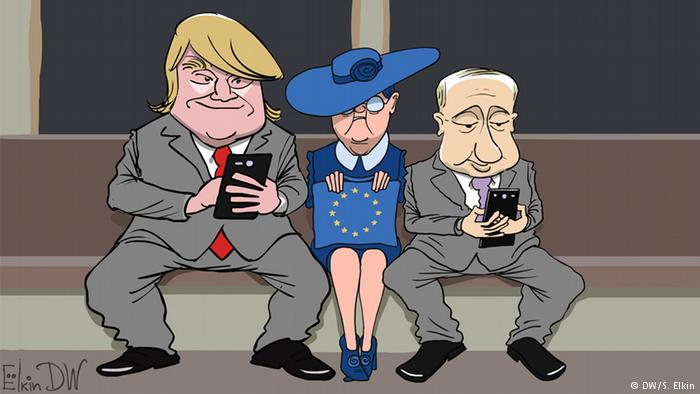
\includegraphics[width=20em,height=10em]{img/putin-trump.jpg}
%%   \caption*{\small\textcopyright Sergey Elkin, Deutsche Welle}
%% \end{figure*}
